% Empirical reliability anchor (Section S8). Written during the journal
% revision (agent S, 2026-10-13) from the SHP paragraphs of sections/results.tex,
% sections/discussion.tex and the ODD of the rule-assembled attempt, the frozen
% protocol of the anchor (shp-reliability-preregistration.md, successor 1) and
% the approved aggregate output of the anchor. Values: v4.shp.* keys; STARTS
% and crosswalk values from the public aggregates (objects.shp, objects.crosswalk);
% counts and fit diagnostics from the approved aggregate of successor 1 (j.shp.* keys).
% Round 4 (2026-10-14): Heise windows (j.shp.heise.*) from the same aggregate; the
% synthetic column of tab:shp-geometry is design arithmetic from Submodel 2
% (7,084 * 0.89^t, plus 3,542 * 0.89^(t-5) from 2004).
% Round 5 (2026-10-14): Heise windows read as eight within j.shp.heise.others.spread
% and a dip of j.shp.heise.dip2003 at the refreshment break, set against the
% free-share shift (j.x3.free.r_shift.*); references for quality (saris2014) and
% attitude-item reliability (alwinkrosnick1991reliability) checked in round5-verification.md;
% the realistic channel shared by both arms stated as a limitation in S8.4.
% Round 6: sensitivity wording with a comparison of scales; the short-lived share
% of the response and the other direction of the share (round6.md item 1).

The anchor places an empirical reliability of the SHP trust item beside the signal-share axis of the simulation. It is secondary and descriptive: it was not used to choose the grid of $r$, the strengths, the targets or any rule, it is not rounded to a grid value, and it does not validate the simulated mechanism.

\subsection{Specification}\label{sec:shp-specification}

The analysis was prespecified on 27 September 2026 and frozen before any SHP microdata were received or accessed; successor 1 was frozen on 28 September 2026, also before access (Section~\ref{sec:odd}, Input data). It was run on the first author's computer, and only aggregate estimates, standard errors, fit statistics and counts left the restricted environment.
\begin{description}
\item[Item and data.] Trust in the federal government in Bern on a 0--10 scale (SHP item \code{P$$P04}), in the eleven annual individual files of 1999--2009 of \emph{Living in Switzerland}, version 12.0 \cite{shpgroup2026data}, linked by the person identifier. Negative codes and empty answers are missing; an answer outside 0--10 would stop the analysis. The protocol notes that the window precedes the alternative interview modes the SHP offered from 2010.
\item[Model.] A quasi-simplex measurement model $Y_{it}=\mu_t+Z_{it}+\epsilon_{it}$ with error centered, independent across waves and independent of the state; $Z_t=\phi Z_{t-1}+\eta_t$ with constant $\phi$ and innovation variance, a free variance of the 1999 state, an error variance equal across waves and free wave means. The reliability of wave $t$ is $r_t=\mathrm{Var}(Z_t)/(\mathrm{Var}(Z_t)+\mathrm{Var}(\epsilon_t))$.
\item[Estimation.] Gaussian full-information maximum likelihood (FIML) over all observed response patterns, including respondents with a single wave, under the assumption that missing answers are missing at random (MAR) given the observed answers and the model; the 0--10 answers are treated as continuous. No weights are used, and the standard errors are model-based, not design-based. The anchor is $r_{2004}$ with a Wald 95\% interval from the observed information.
\item[Specification sensitivities.] For each of the nine consecutive three-wave windows, Heise's reliability $\rho_{12}\rho_{23}/\rho_{13}$ and the Wiley--Wiley reliabilities from unrestricted FIML means and covariances \cite{heise1969,wiley1970}; their minimum--maximum range is a specification range, not a confidence interval. An ordinal sensitivity applies Heise's identity to bivariate polychoric correlations. Two sample sensitivities refit the eleven-wave model on complete cases and on persons with a valid answer before 2004, a proxy for observed entry before the refreshment sample, not an identification of the original sample.
\item[Trait sensitivity (successor 1).] A trait--state--error (STARTS) model $Y_{it}=\mu_t+T_i+S_{it}+\epsilon_{it}$ \cite{kenny1995tse}, with the same sample, scale and estimation, starting values fixed in the code before access, and declared failure rules (non-convergence, an observed information that is not positive definite, a variance below $10^{-4}$ times the mean observed variance, $|\phi|>0.99$, or a reliability outside $(0,1)$); it is reported beside the quasi-simplex anchor and never selected by fit.
\item[Diagnostics.] Convergence, parameter limits, the largest difference between model-implied and complete-case correlations, agreement of the nine windows, and the effects of the sample sensitivities; no model is chosen by information criteria.
\end{description}
The anchor wave, 2004, was fixed as the central wave of the 1999--2009 window. It is also the first wave of the SHP's first refreshment sample \cite{voorpostel2025shp}, so it mixes first interviews with continuing respondents; successor 1 therefore added a description of that wave.

\subsection{Sample and estimates}\label{sec:shp-results}

\paragraph{Sample.}
\resultnum{j.shp.n_any}{14,756} people gave at least one valid answer in 1999--2009, and \resultnum{j.shp.n_complete}{1,822} answered in all eleven waves. The number of valid answers per wave ranged from \resultnum{j.shp.n_wave.min}{5,092} (2003) to \resultnum{j.shp.n_wave.max}{7,831} (2004, when the refreshment sample entered). The pre-2004 sensitivity used \resultnum{j.shp.n_pre2004}{9,096} people. Table~\ref{tab:shp-geometry} sets these counts beside the geometry of the synthetic panels.

\begin{table}[htbp]
\caption[Observation geometry of the synthetic panels and of the SHP trust item]{Observation geometry of the synthetic panels and of the anchor's sample of the SHP trust item, 1999--2009. Synthetic values are design constants or expected counts computed from them (Section~\ref{sec:odd}, Submodel~2); SHP counts are those of the anchor's sample. Source of the SHP counts: Swiss Household Panel (SHP)}\label{tab:shp-geometry}
\centering\footnotesize
\begin{tabular}{@{}>{\raggedright\arraybackslash}p{0.2\textwidth}>{\raggedright\arraybackslash}p{0.36\textwidth}>{\raggedright\arraybackslash}p{0.36\textwidth}@{}}
\toprule
Feature & Synthetic panels & SHP trust item \\
\midrule
People & 10,626 & \resultnum{j.shp.n_any}{14,756} with at least one valid answer \\[2pt]
Entry & 7,084 people in 1999 and 3,542 in 2004 & first valid answer before 2004 for \resultnum{j.shp.n_pre2004}{9,096} people and in 2004 for \resultnum{j.shp.refresh.n}{3,684}; later for the others \\[2pt]
Answers per wave & 7,084 in 1999; expected about 4,445 in 2003, 7,498 in 2004 and 4,187 in 2009 & \resultnum{j.shp.n_wave.min}{5,092} (2003) to \resultnum{j.shp.n_wave.max}{7,831} (2004) \\[2pt]
Answered in all eleven waves & expected about 2,209 & \resultnum{j.shp.n_complete}{1,822} \\[2pt]
Households and exit & two people per household; household retention 0.89 per wave; exit permanent and independent of attitudes & household structure, temporary nonresponse and the selectivity of exit not compared with the design \\
\botrule
\end{tabular}
\end{table}

\paragraph{Quasi-simplex anchor.}
% Moved from sections/results.tex (Empirical reliability anchor) and sections/discussion.tex (DS05).
For \resultnum{v4.protocol.shp.anchor_year}{2004}, the quasi-simplex model estimated the reliability of the SHP trust item at \resultnum{v4.shp.estimate}{0.674}, with a Wald \resultnum{v4.protocol.shp.wald_level}{95}\% interval from \resultnum{v4.shp.wald_lo}{0.667} to \resultnum{v4.shp.wald_hi}{0.682}. The interval is model-based: it uses no weights, treats persons as independent, ignoring their clustering in households, and assumes the quasi-simplex model. The fit converged and no parameter was at a bound; the persistence was \resultnum{j.shp.multiwave.persistence}{0.961}, the wave reliabilities ranged from \resultnum{j.shp.multiwave.r_t.min}{0.670} to \resultnum{j.shp.multiwave.r_t.max}{0.680}, and the largest difference between model-implied and complete-case correlations was \resultnum{j.shp.multiwave.max_cc_residual}{0.078}, so the model does not reproduce every correlation of the item closely. All nine polychoric estimates were admissible. The complete-case and pre-2004 refits gave $r_{2004}=\resultnum{j.shp.complete_case.r2004}{0.688}$ and \resultnum{j.shp.pre2004.r2004}{0.679}.

\paragraph{Heise estimates by window.}
The nine Heise estimates ranged from \resultnum{j.shp.heise.min}{0.625} to \resultnum{j.shp.heise.max}{0.702}; Table~\ref{tab:heise-windows} gives each window with its standard error. The prespecification reads their range as a specification range (Section~\ref{sec:shp-specification}). Under the Heise model's own assumptions, a first-order Markov latent process with independent errors, each window's estimate is the reliability of its middle wave, so the nine values also describe how the estimated reliability varies over 2000--2008; a stable trait would bias them downward, but under stationarity by the same factor in every window. Eight of the nine windows lie within \resultnum{j.shp.heise.others.spread}{0.029} of each other, from \resultnum{j.shp.heise.w1999}{0.673} for 1999--2001 to \resultnum{j.shp.heise.max}{0.702}, rising gently over the decade; at standard errors of \resultnum{j.shp.heise.w2004.se}{0.011} to \resultnum{j.shp.heise.w2002.se}{0.014}, sampling error alone could produce a spread of that size, so neither the spread nor the rise estimates a drift. The exception is the window centered on 2004 (2003--2005), when the refreshment sample entered: at \resultnum{j.shp.heise.min}{0.625}, it lies \resultnum{j.shp.heise.dip2003}{0.065} below the mean of its two neighbors, and with it the spread is \resultnum{j.shp.heise.spread}{0.077}, much wider than the Wald interval of the anchor (\resultnum{v4.shp.wald_lo}{0.667} to \resultnum{v4.shp.wald_hi}{0.682}), which reflects sampling under one model and is itself several times wider than the free-share shift of Section~\ref{sec:x3}. Sampling error, the change in composition in 2004 and dynamics that are not first-order Markov may all contribute; the analysis does not separate them. The window for 2003--2005 and the quasi-simplex anchor for 2004, \resultnum{v4.shp.estimate}{0.674}, rest on different information: the window uses only the three correlations among 2003, 2004 and 2005, whereas the anchor fits all eleven waves with one persistence and one error variance.

Read after the results became available, a change in composition could produce such a dip. If people interviewed for the first time in 2004 answered with more error, the correlations of 2004 with 2003 and with 2005 would fall, but not the correlation between 2003 and 2005, and the window's estimate would fall with them. A gentle rise with a dip when many first interviews enter is also, at a smaller size, the pattern of the declared panel-conditioning channel, in which the signal share rises with the number of earlier interviews (Section~\ref{sec:odd}, Submodel~5); when such conditioning was present in the panels but not in the channel assumed for B, B could not be fitted at any of the nine shares of the grid (Section~\ref{sec:x5}). The free-share fit that removed most of the separation at the boundary moved B's signal share by only \resultnum{j.x3.free.r_shift.min}{0.0011} to \resultnum{j.x3.free.r_shift.max}{0.0028} (Section~\ref{sec:x3}): separation was sensitive to the assumed share in its third decimal, whereas these estimates have standard errors of \resultnum{j.shp.heise.w2004.se}{0.011} to \resultnum{j.shp.heise.w2002.se}{0.014}, a comparison of scales only. What would have to be known at that scale is the short-lived share of the response, error plus any short-lived true component, not the reliability alone: with one answer per wave a slightly lower share is the same as such a component (Section~\ref{sec:x3}), which quasi-simplex models count as error \cite[p.~183]{saris2014}. In the other direction, a share set too high makes B overshoot the panels' lag-three correlation, the sign that influence leaves: \resultnum{j.x3.plus.offset}{0.01} above the design share, B's lag-three correlation exceeded the influence arm's by \resultnum{j.x3.plus.l3_miss.min}{0.0069} to \resultnum{j.x3.plus.l3_miss.max}{0.0081} (Section~\ref{sec:x3}). A drift in the signal share also separates panels without influence: a linear trend from $r-0.03$ in the first wave to $r+0.03$ in the last gave AUCs from \resultnum{j.x5.trend003.min}{0.680} to \resultnum{j.x5.trend003.max}{0.710} and left the same sign pattern in the lag correlations as influence (Section~\ref{sec:x5}). The window estimates are not a test of drift in the item's reliability, and the anchor remains an illustration, not a calibration of the simulation: it shows only that the item's reliability estimates are far coarser than the scale to which separation in this design was sensitive. Like the anchor and its trait sensitivity, these estimates identify reliability through the lag structure of one answer per wave, the structure the classifier reads; evidence on the short-lived share that does not rest on it needs several indicators of the attitude in each wave or measurement repeated within a wave.

\begin{table}[tp]
\caption{Heise reliability by three-wave window for the Swiss Household Panel trust item.}\label{tab:heise-windows}
\centering\scriptsize
\setlength{\tabcolsep}{2pt}
\begin{tabular}{>{\raggedright\arraybackslash}p{42mm}>{\raggedright\arraybackslash}p{36mm}>{\raggedright\arraybackslash}p{42mm}}
\toprule
Window & Estimate & Standard error \\
\midrule
\resultnum{j.shp.heise.w1999.start}{1999}--\resultnum{j.shp.heise.w1999.end}{2001} & \resultnum{j.shp.heise.w1999}{0.673} & \resultnum{j.shp.heise.w1999.se}{0.012} \\
\resultnum{j.shp.heise.w2000.start}{2000}--\resultnum{j.shp.heise.w2000.end}{2002} & \resultnum{j.shp.heise.w2000}{0.675} & \resultnum{j.shp.heise.w2000.se}{0.012} \\
\resultnum{j.shp.heise.w2001.start}{2001}--\resultnum{j.shp.heise.w2001.end}{2003} & \resultnum{j.shp.heise.w2001}{0.691} & \resultnum{j.shp.heise.w2001.se}{0.012} \\
\resultnum{j.shp.heise.w2002.start}{2002}--\resultnum{j.shp.heise.w2002.end}{2004} & \resultnum{j.shp.heise.w2002}{0.697} & \resultnum{j.shp.heise.w2002.se}{0.014} \\
\resultnum{j.shp.heise.w2003.start}{2003}--\resultnum{j.shp.heise.w2003.end}{2005} & \resultnum{j.shp.heise.w2003}{0.625} & \resultnum{j.shp.heise.w2003.se}{0.013} \\
\resultnum{j.shp.heise.w2004.start}{2004}--\resultnum{j.shp.heise.w2004.end}{2006} & \resultnum{j.shp.heise.w2004}{0.684} & \resultnum{j.shp.heise.w2004.se}{0.011} \\
\resultnum{j.shp.heise.w2005.start}{2005}--\resultnum{j.shp.heise.w2005.end}{2007} & \resultnum{j.shp.heise.w2005}{0.702} & \resultnum{j.shp.heise.w2005.se}{0.011} \\
\resultnum{j.shp.heise.w2006.start}{2006}--\resultnum{j.shp.heise.w2006.end}{2008} & \resultnum{j.shp.heise.w2006}{0.695} & \resultnum{j.shp.heise.w2006.se}{0.012} \\
\resultnum{j.shp.heise.w2007.start}{2007}--\resultnum{j.shp.heise.w2007.end}{2009} & \resultnum{j.shp.heise.w2007}{0.702} & \resultnum{j.shp.heise.w2007.se}{0.012} \\
\botrule
\end{tabular}
\par\smallskip\parbox{\linewidth}{Estimates and standard errors are copied from the approved aggregate. Under a first-order Markov latent process and independent errors, each estimate describes the middle wave's reliability. No per-window fit flags are recorded. The minimum is \resultnum{j.shp.heise.min}{0.625}, the maximum is \resultnum{j.shp.heise.max}{0.702}, and their spread is \resultnum{j.shp.heise.spread}{0.077}; this range is not a confidence interval.}
\end{table}


\paragraph{Trait sensitivity.}
The STARTS fit was admissible: none of the declared failure rules applied. It gave $r_{2004}=\resultnum{j.shp.starts.estimate}{0.696}$, with Wald 95\% interval \resultnum{j.shp.starts.wald_lo}{0.685}--\resultnum{j.shp.starts.wald_hi}{0.708}, a persistence of \resultnum{j.shp.starts.persistence}{0.717}, and a stable trait accounting for \resultnum{j.shp.starts.trait_share_2004}{0.758} of the latent variance in 2004. Its reliability is higher than the quasi-simplex anchor, in the direction expected if a stable trait is present, because simplex-type estimators then attribute part of the long-lag plateau to the autoregression. For example, with latent lag correlations $0.5+0.5\cdot0.5^k$ and $r=0.70$, the Heise triplet estimate is about 0.63. % DS05

\paragraph{The 2004 wave.}
In the eleven-wave fit, $r_{2003}=\resultnum{j.shp.wave.r2003}{0.675}$, $r_{2004}=\resultnum{v4.shp.estimate}{0.674}$ and $r_{2005}=\resultnum{j.shp.wave.r2005}{0.673}$. Among the \resultnum{j.shp.refresh.n}{3,684} people whose first valid answer was in 2004, a proxy for entry through the refreshment sample, a quasi-simplex fit over 2004--2009 gave an edge estimate of $r_{2004}=\resultnum{j.shp.refresh.r2004}{0.682}$ (standard error \resultnum{j.shp.refresh.se}{0.010}); because that fit holds the error variance equal across 2004--2009, it does not show whether first interviews carried more error. Both are descriptive and do not replace the anchor.

Table~\ref{tab:shp-estimates} collects these estimates.

\begin{table}[htbp]
\caption[Reliability estimates of the SHP trust item]{Reliability estimates of the SHP trust item for 2004, by specification and sample, from the approved aggregate output of the anchor. The quasi-simplex anchor is the prespecified primary estimate; the other rows are prespecified sensitivities or descriptions and are not selected by fit. Wald intervals are model-based, without weights or allowance for the clustering of persons in households. Source: Swiss Household Panel (SHP)}\label{tab:shp-estimates}
\centering\footnotesize
\begin{tabular}{@{}p{0.38\textwidth}p{0.1\textwidth}p{0.22\textwidth}p{0.2\textwidth}@{}}
\toprule
Specification and sample & $r_{2004}$ & Interval or range & Status \tabularnewline
\midrule
\raggedright Quasi-simplex, eleven waves, all respondents (anchor) & \raggedright \resultnum{v4.shp.estimate}{0.674} & \raggedright Wald \resultnum{v4.shp.wald_lo}{0.667}--\resultnum{v4.shp.wald_hi}{0.682} & \raggedright converged; no parameter at a bound \tabularnewline
\raggedright Heise, nine three-wave windows &  & \raggedright \resultnum{v4.shp.env_lo}{0.625}--\resultnum{v4.shp.env_hi}{0.702} (specification range) & \raggedright middle-wave reliabilities (Table~\ref{tab:heise-windows}) \tabularnewline
\raggedright Polychoric Heise, nine windows &  &  & \raggedright all admissible \tabularnewline
\raggedright Trait--state--error (STARTS) & \raggedright \resultnum{j.shp.starts.estimate}{0.696} & \raggedright Wald \resultnum{j.shp.starts.wald_lo}{0.685}--\resultnum{j.shp.starts.wald_hi}{0.708} & \raggedright admissible \tabularnewline
\raggedright Quasi-simplex, complete cases (\resultnum{j.shp.n_complete}{1,822} people) & \raggedright \resultnum{j.shp.complete_case.r2004}{0.688} &  & \raggedright converged \tabularnewline
\raggedright Quasi-simplex, valid answer before 2004 (\resultnum{j.shp.n_pre2004}{9,096} people) & \raggedright \resultnum{j.shp.pre2004.r2004}{0.679} &  & \raggedright converged \tabularnewline
\raggedright Quasi-simplex over 2004--2009, first valid answer in 2004 (\resultnum{j.shp.refresh.n}{3,684} people; edge estimate) & \raggedright \resultnum{j.shp.refresh.r2004}{0.682} & \raggedright standard error \resultnum{j.shp.refresh.se}{0.010} & \raggedright descriptive \tabularnewline
\botrule
\end{tabular}
\end{table}

\subsection{Synthetic crosswalk}\label{sec:shp-crosswalk}

The crosswalk asks what the anchor estimator returns when the data come from the synthetic generator with known $r$. Successor 1 ran the frozen v4 generator with the SHP-like geometry, coded the eleven categories 0--10 as continuous as in the SHP, and applied the anchor's quasi-simplex estimator to ten panels per cell: the influence arm at $a=0$ (which coincides pathwise with persistence models A, B, D and E at zero strength) and B with $\phi=0.85$ and trait weight $\lambda=0.25$ or 0.50, at every $r$ of the grid, with seeds outside every confirmatory namespace. The declared plan also covered the influence arm at positive strengths, and those cells were computed: the crosswalk record of successor 1 holds the influence arm at every strength and share. As successor 1 declared for the display, the figure and Table~\ref{tab:shp-crosswalk} keep the zero-strength cells and the B references, and the positive-strength cells are not reported here. The table gives the minimum--maximum of the ten estimates per cell; no replicate failed. At zero strength the estimator returned values below the design share at every $r$, so the reliability of the observed 0--10 scores, as this estimator measures it, lies slightly below the signal share of the continuous response. The SHP estimate, \resultnum{v4.shp.estimate}{0.674}, lies in the range of the zero-strength reference only at $r=0.70$ and in no range of either B reference. The ranges depend on the synthetic law and are not confidence intervals: they neither propagate the uncertainty of the empirical anchor nor calibrate $r$ empirically, and they yield no empirically calibrated $a^*(r)$.

\begin{table}[htbp]
\caption[Synthetic crosswalk of the anchor estimator]{Synthetic crosswalk of the anchor estimator: minimum--maximum of the quasi-simplex $r_{2004}$ over ten synthetic panels per cell, by design signal share $r$, for the influence arm at zero strength and for B with trait weight 0.25 and 0.50. No replicate failed. The SHP anchor is \resultnum{v4.shp.estimate}{0.674}. Exploratory; source of the anchor: Swiss Household Panel (SHP)}\label{tab:shp-crosswalk}
\centering\footnotesize
\begin{tabular*}{\textwidth}{@{\extracolsep{\fill}}cccc@{}}
\toprule
$r$ & Zero strength & B, $\lambda=0.25$ & B, $\lambda=0.50$ \\
\midrule
0.50 & \resultnum{j.shp.crosswalk.a0.r050.low}{0.469}--\resultnum{j.shp.crosswalk.a0.r050.high}{0.484} & \resultnum{j.shp.crosswalk.b025.r050.low}{0.461}--\resultnum{j.shp.crosswalk.b025.r050.high}{0.472} & \resultnum{j.shp.crosswalk.b050.r050.low}{0.458}--\resultnum{j.shp.crosswalk.b050.r050.high}{0.470} \\
0.55 & \resultnum{j.shp.crosswalk.a0.r055.low}{0.515}--\resultnum{j.shp.crosswalk.a0.r055.high}{0.527} & \resultnum{j.shp.crosswalk.b025.r055.low}{0.502}--\resultnum{j.shp.crosswalk.b025.r055.high}{0.521} & \resultnum{j.shp.crosswalk.b050.r055.low}{0.498}--\resultnum{j.shp.crosswalk.b050.r055.high}{0.521} \\
0.60 & \resultnum{j.shp.crosswalk.a0.r060.low}{0.564}--\resultnum{j.shp.crosswalk.a0.r060.high}{0.575} & \resultnum{j.shp.crosswalk.b025.r060.low}{0.558}--\resultnum{j.shp.crosswalk.b025.r060.high}{0.567} & \resultnum{j.shp.crosswalk.b050.r060.low}{0.555}--\resultnum{j.shp.crosswalk.b050.r060.high}{0.566} \\
0.65 & \resultnum{j.shp.crosswalk.a0.r065.low}{0.615}--\resultnum{j.shp.crosswalk.a0.r065.high}{0.630} & \resultnum{j.shp.crosswalk.b025.r065.low}{0.604}--\resultnum{j.shp.crosswalk.b025.r065.high}{0.618} & \resultnum{j.shp.crosswalk.b050.r065.low}{0.602}--\resultnum{j.shp.crosswalk.b050.r065.high}{0.616} \\
0.70 & \resultnum{j.shp.crosswalk.a0.r070.low}{0.667}--\resultnum{j.shp.crosswalk.a0.r070.high}{0.679} & \resultnum{j.shp.crosswalk.b025.r070.low}{0.658}--\resultnum{j.shp.crosswalk.b025.r070.high}{0.668} & \resultnum{j.shp.crosswalk.b050.r070.low}{0.655}--\resultnum{j.shp.crosswalk.b050.r070.high}{0.664} \\
0.75 & \resultnum{j.shp.crosswalk.a0.r075.low}{0.715}--\resultnum{j.shp.crosswalk.a0.r075.high}{0.728} & \resultnum{j.shp.crosswalk.b025.r075.low}{0.709}--\resultnum{j.shp.crosswalk.b025.r075.high}{0.717} & \resultnum{j.shp.crosswalk.b050.r075.low}{0.707}--\resultnum{j.shp.crosswalk.b050.r075.high}{0.712} \\
0.80 & \resultnum{j.shp.crosswalk.a0.r080.low}{0.766}--\resultnum{j.shp.crosswalk.a0.r080.high}{0.780} & \resultnum{j.shp.crosswalk.b025.r080.low}{0.761}--\resultnum{j.shp.crosswalk.b025.r080.high}{0.768} & \resultnum{j.shp.crosswalk.b050.r080.low}{0.758}--\resultnum{j.shp.crosswalk.b050.r080.high}{0.766} \\
0.85 & \resultnum{j.shp.crosswalk.a0.r085.low}{0.817}--\resultnum{j.shp.crosswalk.a0.r085.high}{0.828} & \resultnum{j.shp.crosswalk.b025.r085.low}{0.813}--\resultnum{j.shp.crosswalk.b025.r085.high}{0.821} & \resultnum{j.shp.crosswalk.b050.r085.low}{0.810}--\resultnum{j.shp.crosswalk.b050.r085.high}{0.819} \\
0.90 & \resultnum{j.shp.crosswalk.a0.r090.low}{0.869}--\resultnum{j.shp.crosswalk.a0.r090.high}{0.882} & \resultnum{j.shp.crosswalk.b025.r090.low}{0.866}--\resultnum{j.shp.crosswalk.b025.r090.high}{0.874} & \resultnum{j.shp.crosswalk.b050.r090.low}{0.865}--\resultnum{j.shp.crosswalk.b050.r090.high}{0.871} \\
\botrule
\end{tabular*}
\end{table}

\subsection{What the anchor shows and what it does not}\label{sec:shp-reading}

% Moved from sections/discussion.tex (DS05) and sections/results.tex.
The anchor and the simulation's signal share are different quantities. The anchor treats the 0--10 responses as continuous, whereas $r$ is the signal share of a continuous channel before rank-based discretization into eleven equiprobable categories; the anchor model is a latent autoregression without a stable trait, while B includes one; the anchor wave mixes first interviews with continuing respondents; and its interval is model-based. The raw quasi-simplex anchor, the STARTS sensitivity and the synthetic compatibility set must therefore be read separately. % DS05 RC24 RC25 RC26
The synthetic panels approximate the SHP's size and refreshment design, not its persistence (Table~\ref{tab:shp-geometry}): they have fewer people than the anchor's sample, every household has two people, entry happens only in 1999 and 2004, and exit is permanent and independent of attitudes. The lag profile of the trust item, its heaping at 0, 5 and 10 and its attrition pattern were never compared with the synthetic panels. Nor was a channel with such heaping and with error largest near the middle of the scale applied to both arms with B correctly specified: model C gave midpoint heaping and such error to its persistence arm only (Section~\ref{sec:odd}, Submodel~5), so the boundary under a realistic channel shared by both arms is unknown. The generator has no stable trait (at $a=0$ the influence arm is model A with $\phi=0.85$), whereas the STARTS fit puts \resultnum{j.shp.starts.trait_share_2004}{0.758} of the item's latent variance in 2004 in a stable trait; the resemblance to the SHP therefore concerns size and refreshment design only. The aggregate output of the anchor records the shares of answers at 5 and at the endpoints by wave, but no comparison was declared or made. Item, mode and reliability estimand differ across published surveys, and the reliability of attitude items varies with question format and respondent attributes \cite{alwinkrosnick1991reliability}, so external reliability estimates cannot be assigned to this item without item-specific evidence \cite{antoun2026,lucasdonnellan2012}.
Read after the results became available, the anchor allows only a conditional, illustrative statement; it does not calibrate the simulation and gives no estimated threshold for the SHP item. Under this synthetic generator and its observation channel, the grid shares nearest the anchor, $r=0.65$ and 0.70, gave a first boundary against B of $a=\resultnum{j.b.r065.first.point}{0.10}$, with the response channel correctly specified, $r$ known and persistence of the trait-plus-autoregressive form. Two findings make even this conditional reading optimistic. Letting B fit its own signal share while matching lag three, with the discriminator reduced to lags four and five, lowered the AUC at the boundary cell at every share, through a fit that moved the share by only \resultnum{j.x3.free.r_shift.min}{0.0011} to \resultnum{j.x3.free.r_shift.max}{0.0028}, far below the standard errors of this item's three-wave reliability estimates (Sections~\ref{sec:x3} and~\ref{sec:shp-results}). And a misspecified channel alone separates panels without influence, leaving the same sign pattern in the lag correlations as influence (Section~\ref{sec:x5}). Where the item lies on the design's scale is also uncertain in a way the anchor cannot settle. Quasi-simplex and trait--state--error reliabilities count a stable response style as signal, because it enters the state or the trait, whereas the design treats persistent style as error (Section~\ref{sec:odd}, Submodel~5); measurement quality, the share of the response variance explained by the latent trait of interest \cite{poses2021,saris2014}, is closer to $r$ in that respect, and by this route the anchor would overstate the item's signal share. Without such style, the crosswalk shows the opposite: the estimator returns slightly less than the design share (Section~\ref{sec:shp-crosswalk}). The net direction is unknown; at $r=0.50$ the first boundary against B was $a=\resultnum{j.b.r050.first.point}{0.30}$.
Figure~\ref{fig:shp-anchor} displays the empirical reliability summaries, that is, the quasi-simplex anchor with its Wald interval, the specification range of the Heise estimates and the STARTS sensitivity with its Wald interval, on the signal-share axis of the design; Table~\ref{tab:shp-crosswalk} reports the synthetic crosswalk. Nothing is interpolated or extrapolated.

\begin{figure}[tp]
\centering
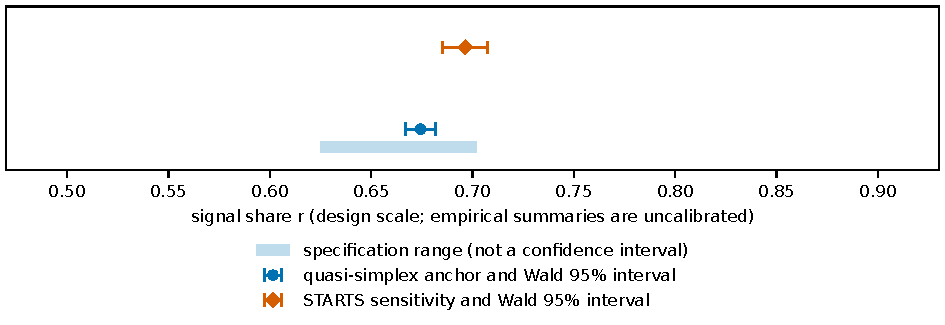
\includegraphics[width=\textwidth]{generated/J6_shp_anchor.pdf}
\caption{Reliability summaries for the Swiss Household Panel trust item. The quasi-simplex anchor and the STARTS point estimate refer to the \resultnum{v4.protocol.shp.anchor_year}{2004} wave and have Wald 95\% intervals. The shaded specification range spans the nine Heise triplet estimates over 1999--2009, from \resultnum{v4.shp.env_lo}{0.625} (2003--2005) to \resultnum{v4.shp.env_hi}{0.702} (2007--2009); it is not a confidence interval. The anchor is placed on the signal-share axis without calibrating it to the design.}\label{fig:shp-anchor}
\end{figure}


\clearpage
